
\subsection{Technische Aspekte für unser Experiment}
In unserem Fall besteht die Spitze des RTMs aus einer möglichst spitzen
Drahtspitze, durch die der Tunnelstrom geleitet wird. Dazu wird an die Spitze eine
Tunnelspannung angelegt und so nahe an die Probe angenähert, bis der Tunnelstrom
im nA-Bereich fliessen kann.
Nun gibt es zwei verschiedene Modi, über die das RTM verfügt:
\begin{itemize}
\item Konstante Höhe (\textit{Constant Height Mode, CHM}): Die Höhe der Spitze wird konstant
gehalten und die Topographie wird anhand der variierenden Tunnelstromstärke ermittelt. Hierbei
entsteht allerdings die große Gefahr, dass die Spitze mit der Oberfläche kollidiert und somit
abbricht bzw. zu Schaden kommt.
\item Konstante Tunnelstromstärke (\textit{Constant Current Mode, CCM}): Hier wird über einen
Regler die Position der Spitze dergestalt verändert, dass immer ein konstanter Tunnelstrom
fliessen kann. Die Topographie der Probe erhalten wir über das Ausgangssignal des Reglers.
Dies ist die empfohlene Einstellung und diese werden wir auch benutzen.
\end{itemize}
Dies erfordert eine ziemlich präzise Steuerung der Spitze, welche nun weiter erläutert wird.
Der Tunnelstrom muss einerseits konstant gehalten werden (jedenfalls nach der gängigen Methode),
andererseits darf die Distanz nicht zu schnell geändert werden, da sonst eine Kollision mit der
Probe stattfindet. Dafür gibt es einen Regelkreis, der kontinuierlich den angegeben Wert
(Führungsgröße) mit dem
tatsächlichen Wert (Regelgröße) vergleicht und
die Steuerung daraufhin verändert. Hier wird ein PID-Regler
eingesetzt, welcher auch bei Störeinflüssen seine Funktion, den Strom konstant zu halten,
noch erfüllt, wenn die Störungen nicht zu hoch sind. Im Allgemeinen existieren viele
verschiedene Regler, die für verschiedene Verhaltensformen des Signals angepasst sind.
Hierfür wollen wir eine kurze Einführung in die Kinematik geben \cite{regelungstechnik}.
\subsubsection{Einführung in die Kontrolltheorie und Kinematik: PID-Regler}
Die Kontrolltheorie beschäftigt sich mit der Beeinflussung von Systemen, um bestimmten
Ausgangsgrößen einen gewünschten zeitlichen Verlauf aufzuprägen\cite{regelungstechnik}.
Der gewünschte zeitliche Verlauf der Ausgangsgrößen wird durch die Sollgrößen oder Sollwerte
definiert. Eingangsgröße der Steuerung ist also der Sollwert $w$, ihre Ausgangsgröße ist die
Stellgröße $u$, welche zusammen mit der Störgröße $d$ wieder eine Eingangsgröße bildet. Die
Anforderungen an die Regelung sind klar: Die Regelabweichung soll im stationären Zustand
nach Beendigung
eines Einschwingvorgangs möglichst klein sein, im Falle einer Führungsgrößenänderung oder einer
Störung soll die entstandene Regelabweichung möglichst schnell wieder eliminiert werden und
Die Stabilität des Gesamtsystems muss durchgehend gewährtleistet werden.
Die \textit{Laplace-Transformation}\cite{regelungstechnik2} dient als wichtigstes Hilfsmittel
bei regelungstechnischen Aufgaben, die mit Differenzialgleichungen beschrieben werden können; dies
ist insbesondere beim PID-Regler der Fall. Die Laplace-Transformation wird folgendermaßen definiert:
\begin{align}
F(s) &= \mathcal{L}\left [f(t)\right ] = \int_{0}^{\infty}f(t)e^{-st}dt \\
f(t) &= \mathcal{L}^{-1}\left [F(s)\right ] =
\frac{1}{2\pi i} \int_{c - i\infty}^{c+ i\infty} F(s)e^{st}ds
\end{align}
Wobei als Argument die komplexe Variable $s=\sigma + i\omega$ auftritt (somit handelt es sich
bei der schon erwähnten Fourier-Transformation um einen Spezialfall mit $F(s = ik)$) und
das vorkommende $c\in \mathbb{R}$ so gewählt werden muss, dass der Integrationsweg in der
Konvergenzhalbebene längs einer Parallelen zur imaginärenAchse im Abstand $c$ verläuft, wobei
$c$ größer als die Realteile sämtlicher singulärer Punkte von $F(s)$ sein muss.
Hier die wichtigsten Eigenschaften der Laplace-Transformation:
\begin{align}
&\mathcal{L}\left [a f(t) + b g(t)\right ]
= a F(s) + b G(s)
&\mbox{ (Linearität) }\\
&\mathcal{L}\left [f(at)\right ]
= \frac{1}{a}F(\frac{s}{a})
&\mbox{ (Ähnlichkeit) }\\
&\mathcal{L}\left [f(t-a)\right ]
= \frac{1}{a}F(\frac{s}{a})
\mbox{ (Translation) }\\
&\mathcal{L}\left [\frac{d^nf(t)}{dt^n}\right ]
= s^nF(s) - \sum_{i=1}^{n}s^{n-i}\frac{d^{i-1}f(t)}{dt^{i-1}}
&\mbox{ (Differentiation) }\\
&\mathcal{L}\left [\int_{0}^{t}f(\tau)d\tau\right ]
= \frac{1}{s}F(s)
&\mbox{ (Integration) }\\
&\mathcal{L}\left [f(t) * g(t)\right ]
= \mathcal{F}\left [f(t)\right ]\mathcal{F}\left [g(t)\right ]
&\mbox{ (Faltungseigenschaft) }
\end{align}
Mit den hier beschriebenen Eigenschaften bietet die Transformation eine sehr
elegante Möglichkeit zur schnellen und schematischen Lösung von linearen Differenzialgleichungen
mit konstanten Koeffizienten (siehe Abbildung~\ref{fig:laplace1}).
\begin{figure}[h]
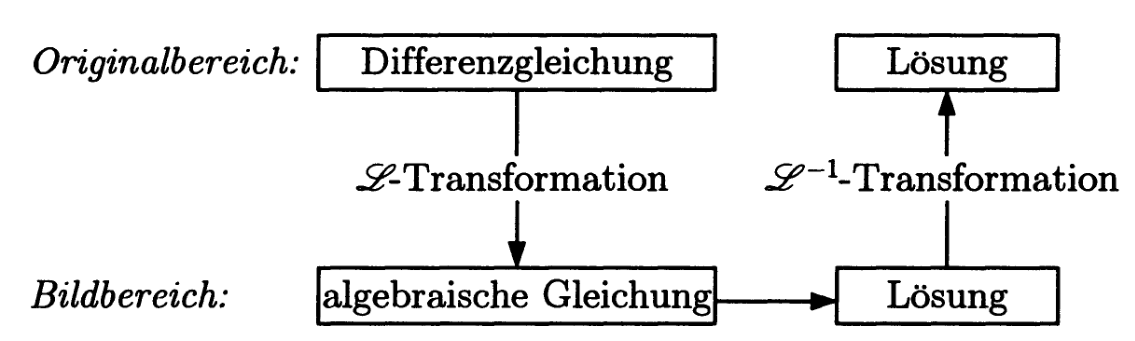
\includegraphics[width=14cm]{pics/laplace1}
\caption{Schema zur Lösung von Differenzialgleichungen mit der Laplace-Transformation
\cite{regelungstechnik2}}
\label{fig:laplace1}
\end{figure}
Der Grund, wieso wir die Laplace-Transformation eingeführt haben, kommt daher, dass wir
die Beziehung zwischen der Führungs- und der Regelgröße (im Idealfall) mit einer
Differenzialgleichung beschreiben können.
Bei einem Eingangssignal $u(t)$ ergibt sich das Ausgangssignal $y(t)$ durch ein
Übertragungsverhalten, welches durch einen Operator $\mathbb{T}$ charakterisiert ist.
Die Gewichtsfunktion sei nun die Lösung des Operators unter Einsetzen der Deltafunktion:
\begin{align}
y(t) &= T\left [ u(t) \right ] \\
g(t) &= T \left [ \delta(t) \right ] \\
\Rightarrow y(t) &= u(t) * g(t) = \int_{0}^{t}g(t-\tau)u(\tau)d\tau
\end{align}
Mithilfe der Laplacetransformation lässt sich nun die \textit{Übertragungsfunktion} $G(s)$
des Systems definieren:
definieren:
\begin{align}
y(t) &= u(t) * g(t) \\
\Leftrightarrow \mathcal{L}\left [y(t)\right ] &= \mathcal{L}\left [u(t) * g(t)\right ]\\
\Leftrightarrow Y(s) &= U(s)G(s)
\end{align}
Ausgehend hiervon lassen sich nun Übertragungsfunktionen zu Übertragungssystemen kombinieren:
\begin{itemize}
\item Reihenschaltung: $G(s) = G_1(s)G_2(s)$
\item Paralellschaltung: $G(s) = G_1(s) + G_2(s)$
\item Kreisschaltung: $\frac{G_1(s)}{1\pm G_1(s)G_2(s)}$
\end{itemize}
Nun können wir die verschiedenen Glieder P,I und D aufstellen, die den PID-Regler ausmachen.
Die Glieder reagieren jeweils auf eine Regelabweichung $e(t)$:
\paragraph{Das P-Glied} reagiert proportional zum Eingangssignal mit einer Verstärkung $K_R$:
\begin{equation}
u(t) = K_p e(t) \Rightarrow G(s) = K_R
\end{equation}
\paragraph{Das I-Glied} integriert die Regelabweichung $e(t)$ über eine Nachstellzeit $T_N$ auf:
\begin{equation}
u(t)= \frac{1}{T_I}\int_{0}^{t}e(\tau)d\tau \Rightarrow G(s) = \frac{1}{sT_I}
\end{equation}
\paragraph{Das D-Glied} differenziert die Regelabweichung, reagiert also auf die
Änderungsgeschwindigkeit mit einem Proportionalitätsfaktor $T_D$:
\begin{equation}
u(t) = T_D \frac{d}{dt}e(t) \Rightarrow G(s) = s T_D
\end{equation}
Diese Glieder ergeben kombiniert untereinander noch weitere Möglichkeiten, auf die wir
hier jetzt nicht eingehen werden.
Der PID-Regler (\textit{proportional-integral-derivative controller}) besteht nun aus Anteilen
aus allen drei Gliedern. Er kann sowohl in einer Parallel- als auch Reihenschaltung aufgebaut
werden. Die Differenzialgleichung und die Übertragungsfunktion
für den idealen PID-Regler (Reihenschaltung) lauten somit:
\begin{align}
u(t) &= K_P \left( e(t) + \frac{1}{T_I} \int_{0}^{t} e(\tau) d\tau + T_D \frac{d}{dt} e(t) \right)\\
G(s) &= K_P \frac{1 + s T_I + s^2 T_I T_D}{S T_I}
\end{align}
Der Regler reagiert somit auf eine eine zu hohe Abweichung des Werts an sich (P-Glied), auf einen
zu hohen Wert integriert über die Zeit (I-Glied) und auf eine zu hohe Änderung der Abweichung
(D-Glied). Somit ist er recht anpassungsfähig und kann auf verschiedene Szenarien, sofern sie sich
im linearen Regime bewegen, sehr gut reagieren. Durch diese \textit{Feedback} Mechanismen wird
er sehr häufig in industriellen Systemen angewandt. Vor allem wenn über die unterliegende
Dynamik der Eingangsvariable nur unzureichend Wissen verfügbar ist, wird er als der beste
Regler angesehen. Um eine geeignete Steuerung aufzubauen, werden allerdings noch mehr Kombinationen
der oben beschriebenen Glieder verwendet, das Grundprinzip bleibt allerdings dasselbe.\\
Beim RTM hängen die freien Variablen des Reglers von der Beschaffenheit der Spitze und der Probe
ab, sollten allerdings nicht zu hoch gewählt werden, weil der Regler und die Spitze zusammen
einen Regelkreis mit eigene Eigenfrequenz bilden und sich gegenseitig aufschaukeln können.
Bei unserer Aufnahme mit dem RTM werden innerhalb des Programms zwei Ausgänge visualisiert:
Zum einen der Reglerausgang, der zeigt, wie der Regler den Tunnelstrom konstant hält, dieser
Ausgang zeigt uns im Idealfall die Topographie der Fermioberfläche der Probe; zum anderen sehen
wir als Ausgang den Tunnelstrom. Theoretisch sollte nun dieser Tunnelstrom durch den Regler
konstant gehalten werden, dies ist jedoch nur in der Theorie so. In der Praxis sehen wir
Diskontinuitäten, welche dadurch entstehen, dass der Regler nicht schnell genug oder gegeben
durch die Komplexität der Oberfläche die Position der Spitze anpassen kann.
\subsubsection{Piezoelemente und Höheneinstellung}
Die Ausgangsfunktion des Reglers sind im wesentlichen Piezoelemente, welche die Spitze in alle
drei Richtungen bewegen können. Diese bestehen meistens aus piezoelektrischen Keramiken, die also
den Piezoeffekt ausnutzen. Dieser beschreibt die Änderung der elektrischen Polarisation
unter elastischer Verformung und umgekehrt, die Änderung der Verformung durch Anlegen einer
Spannung. Piezoelemente werden hier eingesetzt, weil sich mit ihnen Veränderungen der Position
der Spitze im pm-Bereich ausführen lassen (siehe Abbildung~\ref{fig:piezoeffekt}).
\begin{figure}[h]
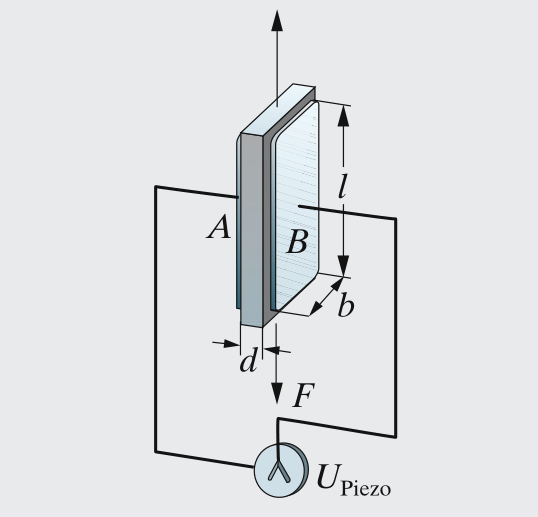
\includegraphics[width=10cm]{pics/piezoeffekt}
\caption{Transversaler Piezoeffekt am Quarzkristall (aus \cite{vogel1997gerthsen}).
Das Piezoelement verändert nun seine Länge senkrecht zur Feldrichtung, das liegt daran, dass der
Quarzkristall eine ausgezeichnete Polare Achse hat.
}
\label{fig:piezoeffekt}
\end{figure}
Wie wir schon gesehen haben, gilt für den Tunnelstrom:
\begin{equation}
I \sim \exp(-kz)
\end{equation}
wobei $k$ eine Konstante und $z$ die Höhe darstellt. Somit regelt der PID-Regler die Höhe durch
die Piezoelemente so, dass sie exponentiell zur Veränderung der Stromstärke angepasst wird.
Durch die Steuerung der Piezoelemente erhalten wir dann auch sofort die Topographie der
Fermidichte an der Oberfläche der Probe.

